\documentclass{beamer}
\usepackage[utf8]{inputenc}

\usetheme{Madrid}
\usecolortheme{default}
\usepackage{amsmath,amssymb,amsfonts,amsthm}
\usepackage{txfonts}
\usepackage{tkz-euclide}
\usepackage{listings}
\usepackage{adjustbox}
\usepackage{array}
\usepackage{tabularx}
\usepackage{gvv}
\usepackage{lmodern}
\usepackage{circuitikz}
\usepackage{tikz}
\usepackage{graphicx}

\setbeamertemplate{page number in head/foot}[totalframenumber]

\usepackage{tcolorbox}
\tcbuselibrary{minted,breakable,xparse,skins}



\definecolor{bg}{gray}{0.95}
\DeclareTCBListing{mintedbox}{O{}m!O{}}{%
  breakable=true,
  listing engine=minted,
  listing only,
  minted language=#2,
  minted style=default,
  minted options={%
    linenos,
    gobble=0,
    breaklines=true,
    breakafter=,,
    fontsize=\small,
    numbersep=8pt,
    #1},
  boxsep=0pt,
  left skip=0pt,
  right skip=0pt,
  left=25pt,
  right=0pt,
  top=3pt,
  bottom=3pt,
  arc=5pt,
  leftrule=0pt,
  rightrule=0pt,
  bottomrule=2pt,

  colback=bg,
  colframe=orange!70,
  enhanced,
  overlay={%
    \begin{tcbclipinterior}
    \fill[orange!20!white] (frame.south west) rectangle ([xshift=20pt]frame.north west);
    \end{tcbclipinterior}},
  #3,
}
\lstset{
    language=C,
    basicstyle=\ttfamily\small,
    keywordstyle=\color{blue},
    stringstyle=\color{orange},
    commentstyle=\color{green!60!black},
    numbers=left,
    numberstyle=\tiny\color{gray},
    breaklines=true,
    showstringspaces=false,
}
%------------------------------------------------------------
%This block of code defines the information to appear in the
%Title page
\title %optional
{1.6.8}
\date{August  2025}
%\subtitle{A short story}

\author % (optional)
{Tangellapalli Mohana Krishna Sushma - EE25BTECH11058}



\begin{document}


\frame{\titlepage}
\begin{frame}{Question}
If three points $\,(x, -1),\, \vec{(2, 1)}\, \text{and} \, \vec{(4, 5)}\,$ are collinear, find the value of $x$.


\end{frame}
 
\begin{frame}{given data}

\[
\begin{array}{|c|c|c|}
\hline
\textbf{Point} & \textbf{x} & \textbf{y} \\
\hline
A & x & -1 \\
B & 2 & 1 \\
C & 4 & 5 \\
\hline
\end{array}
\] 

\end{frame}

\begin{frame}{Formula}
  collinearity matrix can be expressed as 

\begin{align*}
  \begin{myvec}{A-B & A-C\\}\end{myvec}=\begin{myvec}{x-2 & x-4\\-2 & -6\\}\end{myvec}
\end{align*}
\end{frame}

\begin{frame}{allowframebreaks}
\frametitle{Row reduction}

$\myvec{x-2 & x-4\\-2 & -6}
R_2 \leftrightarrow R_1 \implies \myvec{ -2 & -6 \\ x-2 & x-4 }$

$\myvec{ -2 & -6 \\ x-2 & x-4 }
R_2 \rightarrow R_2 + ((x-2)/2)*R_1 \implies \myvec{ -2 & -6 \\ 0 & -2x+2 }$

To make the following matrix Rank 1. (i.e., To prove collinearity)
Thus, we make the bottom row elements zero.

\end{frame}


\begin{align*}
-2x + 2 = 0 \\
\Rightarrow x = 1 \\
\end{align*}

Hence, The value of x = 1.


\begin{frame}[fragile]
    \frametitle{Python Code}
    \begin{lstlisting}
    
import matplotlib.pyplot as plt

# Coordinates of the points
points = {'A': (1, -1), 'B': (2, 1), 'C': (4, 5)}


     \end{lstlisting}
\end{frame}

\begin{frame}[fragile]
    \frametitle{Python Code}
    \begin{lstlisting}
# Extract x and y coordinates separately
x = [coord[0] for coord in points.values()]
y = [coord[1] for coord in points.values()]


     \end{lstlisting}
\end{frame}


\begin{frame}[fragile]
    \frametitle{Python Code}
    \begin{lstlisting}

    
# Plot the points
plt.scatter(x, y, color='deepskyblue', label='Points')

# Annotate each point with its label
for label, (x_coord, y_coord) in points.items():
    plt.annotate(label, (x_coord, y_coord), textcoords="offset points", xytext=(5,-10), ha='center')

# Plot the line through the points
plt.plot(x, y, color='red', label='Line')

# Label axes
plt.xlabel('x')
plt.ylabel('y')
plt.title('Collinear Points with Labels')

# Display legend
plt.legend()

# Show grid
plt.grid(True)

# Show plot
plt.show()

     \end{lstlisting}
\end{frame}

\begin{frame}[fragile]
\frametitle{C Code}
\begin{lstlisting}
#include <stdio.h>

int main() {

    double y1 = -1.0;
    double x2 = 2.0, y2 = 1.0;
    double x3 = 4.0, y3 = 5.0;
    double x1;
    double numerator = y1 * (x2 - x3) - (x2 * y3 - x3 * y2);

    double denominator = y2 - y3;

    x1 = numerator / denominator;

    printf("Using the matrix determinant method for collinear points:\n");
    printf("The value of x is: %.1f\n", x1);

return 0;
}

\end{lstlisting}

\end{frame}

\begin{frame}[fragile]
\frametitle{Python and C Code}

\begin{lstlisting}

import subprocess

# 1. Compile the C program
subprocess.run(["gcc", "collinear.c", "-o", "collinear"])

# 2. Run the compiled C program
result = subprocess.run(["./collinear"], capture_output=True, text=True)

# 3. Print the output from the C program
print(result.stdout)

\end{lstlisting}

\end{frame}

\begin{figure}
    \centering
    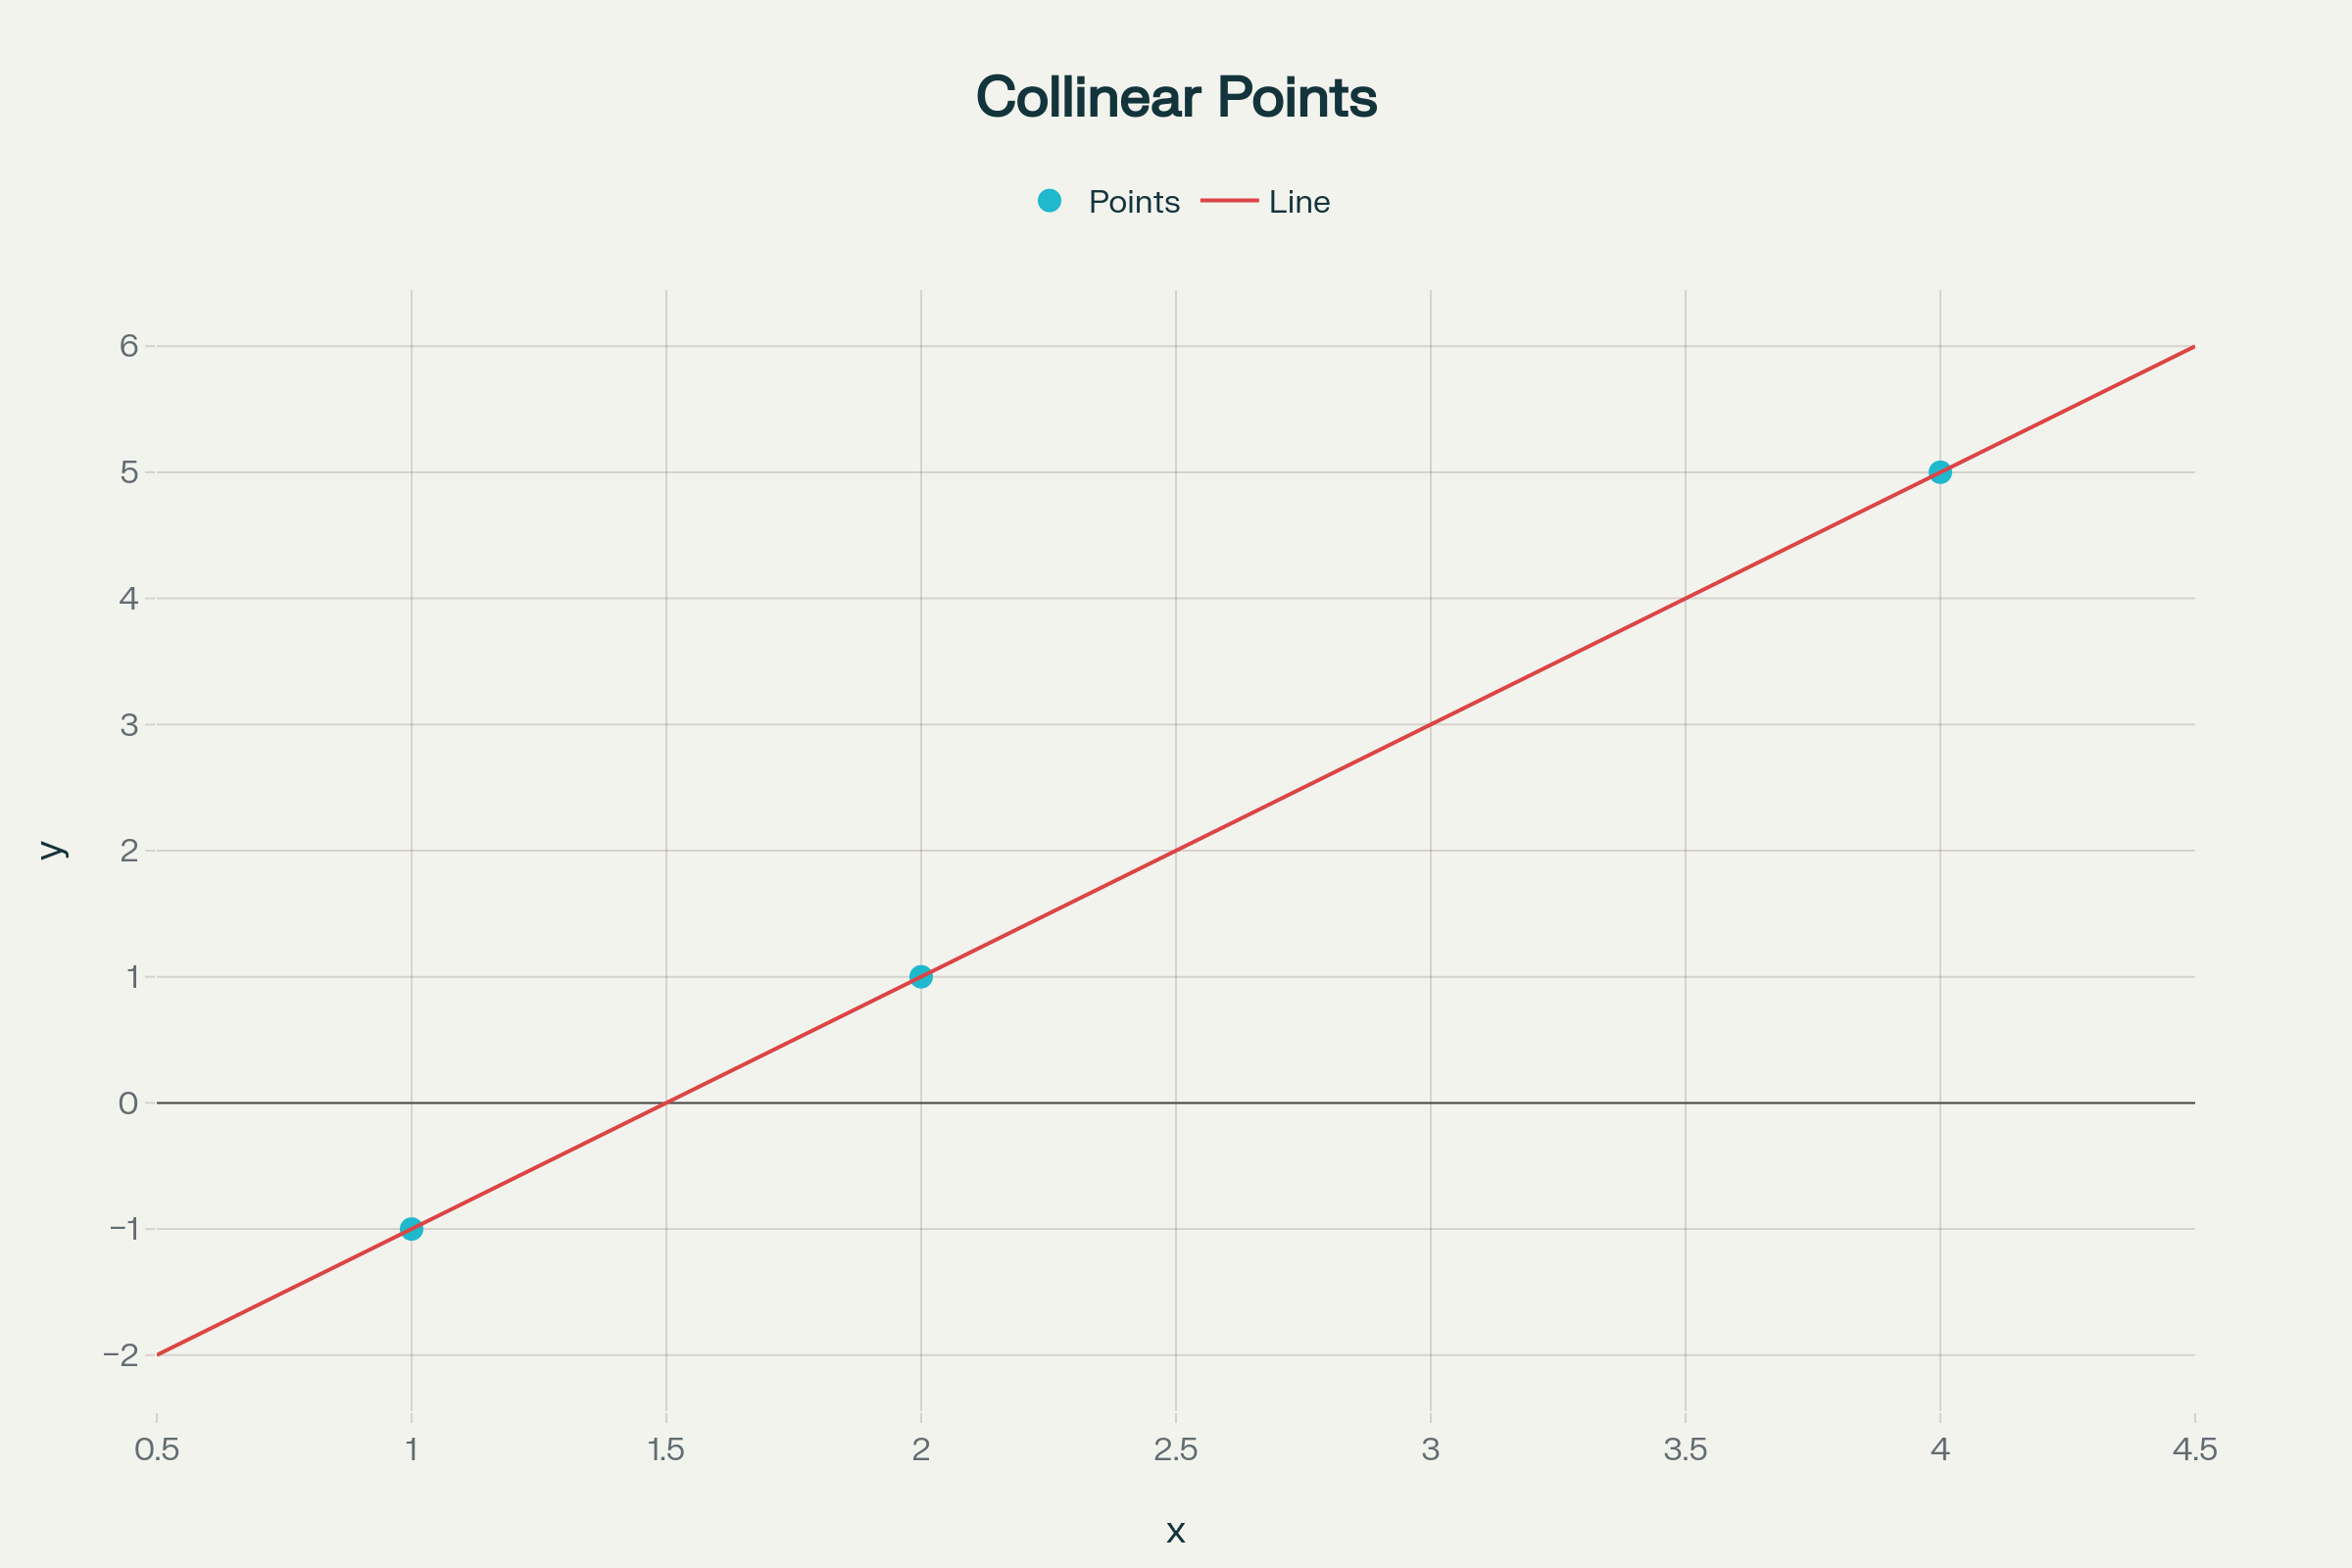
\includegraphics[width=0.8\columnwidth]{figs/fig.png}
    \caption{Collinearity}
    \label{fig:placeholder}
\end{figure}




















\end{document}